\documentclass[utf8, 11pt]{feuille}

\newcommand{\titredutd}{\textbf{Seconde session - 2 h 30 --- Mercredi 10 mai 2023}}

\begin{document}

Seules les calculatrices non communicantes, les notes manuscrites personnelles, les formulaires et les dictionnaires de langues sont autorisées. Les exercices sont totalement indépendants. Comme d'habitude, l'énoncé est probablement trop long pour la durée impartie: concentrez vous sur ce que vous savez faire.

On notera $k_B$ la constante de Boltzmann et $h$ la constante de Planck.



%__________________________________________________________________________________


\section{Extensivité, paradoxe de Gibbs et entropie de mélange}

Nous voulons clarifier le rôle de l’indiscernabilité dans le calcul de l’entropie du gaz parfait classique.

\question Rappeler ce qu'est la propriété d’extensivité pour une grandeur thermodynamique. Comment la vérifier sur l'entropie $S$ à partir de son expression $S(E,V,N)$ en fonction de l'énergie $E$, du volume $V$ et du nombre $N$ de particules du système. 

%\medskip

\begin{center} \vspace{-0.5cm}\line(1,0){0.2\textwidth} \vspace{-0.5cm}\end{center}

On rappelle que  le volume $\Phi$ dans l'espace des phases des états d'énergie inférieure ou égale à $E$ pour un ensemble de $N$ atomes de masse $m$ sans interactions confinés dans un volume $V$ en 3D est de la forme:
\begin{center}
$\Phi(E,V,N)=V^N \frac{(2\pi m E)^\frac{3N}{2}}{(\frac{3N}{2})!}$    
\end{center}

\question En déduire pour des atomes indiscernables le nombre $\phi$ de micro-états d'énergie inférieure ou égale à $E$, puis l'entropie microcanonique de ce gaz (formule de Sackur-Tetrode). Vérifier que l'expression est bien extensive.

\question Rappeler comment obtenir l'expression de la température $T$ et de la pression $P$ d'un système en fonction de son entropie microcanonique $S(E, V, N)$.
Exprimer $T$ et $P$ pour un gaz parfait monoatomique d'énergie $E$, de volume $V$ et à $N$ atomes.
\question En déduire une expression de l'entropie microcanonique uniquement en fonction de $T, P$ et $N$.

%\medskip

\begin{center} \vspace{-0.5cm}\line(1,0){0.2\textwidth} \vspace{-0.5cm}\end{center}

\`A la fin du XIXème siècle, il n’y avait pas de justification pour introduire dans le calcul précédent le facteur $1/N!$  nécessaire pour prendre en compte l’indiscernabilité des atomes. 

\question Donner l’expression de l’entropie microcanonique si les atomes étaient discernables (sans facteur $1/N!$).

\begin{center} \vspace{-0.5cm}\line(1,0){0.2\textwidth} \vspace{-0.5cm}\end{center}

{\sffamily\bfseries{Paradoxe de Gibbs}}
On considère deux gaz monoatomiques identiques (chacun d'énergie $E$, de volume $V$ et à $N$ atomes) occupant deux volumes égaux séparés par une paroi. 

\question Justifier que lorsqu’on enlève la paroi, l’entropie du système varie de $\Delta S_D = S(2E, 2V, 2N)-2S(E, V, N)$ et calculer cette variation. Pourquoi ce résultat est-il paradoxal ? Qu'aurait donné l'utilisation de la formule de Sackur-Tétrode ?

\begin{center} \vspace{-0.5cm}\line(1,0){0.2\textwidth} \vspace{-0.5cm}\end{center}

{\sffamily\bfseries{Entropie de mélange}}

On considère deux gaz monoatomiques non identiques, notés 1 et 2 (le gaz $i$ a une énergie $E_i$, un volume $V_i$ et $N_i$ atomes) occupant deux volumes séparés par une paroi mobile et diatherme.

\medskip

\question On considère qu'ils sont à l'équilibre mécanique et thermique. Que cela signifie-t-il ? On note $T$ la température et $P$ la pression dans chaque compartiment.

\question Calculer l'entropie de ce système avec la paroi en place en fonction de  $T$, $P$, $N_1$ et $N_2$.

\question On enlève la paroi. Que deviennent la température et la pression du système entier, mélange des deux gaz ?

\question Quelle est la pression partielle $P_1$ (respectivement $P_2$) du gaz 1 (resp. 2) ? En déduire l'entropie du système sans la paroi.

\question Calculer la variation d'entropie lorsque l'on a enlevé la paroi. Montrer qu'elle s'exprime comme

\mbox{$\Delta S = - k_B N \{ x \ln{x}+(1-x) \ln{(1-x)} \}$} où $N=N_1+N_2$ et $x=N_1/N$.

\question Pourquoi $\Delta S$ est ici non nul ?


\section{\'Equation d'état d'un gaz parfait selon la statistique}

La figure ci-dessous présente les équations d'état de trois gaz parfaits non relativistes à trois
dimensions (numérotées de haut en bas). Les $N$ particules de masse $m$, confinées dans un volume $V$ sont supposées sans
structure interne. Le produit $pV$ et la température $T$ sont adimensionnés grâce à la température
caractéristique : $T_0=\frac{h^2}{2\pi m k_B} \left( \frac{N}{V} \right)^{\frac{2}{3}}.$
Presqu'aucun calcul n'est attendu dans cet exercice. Des réponses courtes mais précises, de quelques lignes peuvent suffire. On rappelera ce que la définition des fermions et des bosons.

\question Rappeler la définition de la longueur d'onde de De Broglie $\Lambda$ à la température $T$.
Quel est son sens physique ? En déduire une interprétation de la température caractéristique $T_0$.

\question \`A quelle statistique étudiée en cours chacune de ces trois courbes correspond-elle ?

\question Expliquer l'existence d’une ordonnée à l’origine non nulle pour la courbe 1. Donner un exemple de système physique qui vérifie cette équation d'état.

\question Concernant la courbe 3, à quel phénomène physique la température $T^*=\frac{T_0}{\zeta(\frac{3}{2})^{\frac{2}{3}}} \approx  0,52 \ T_0$ (indiquée par un trait vertical sur la figure) correspond-elle ? $\zeta(s)=\sum_{k=1}^{+\infty} \frac{1}{k^s}$ est la fonction zêta de Riemann. 

\question Pour $T \gg T_0$, les trois courbes se rejoignent. En pratique, la courbe 2 est-elle réaliste à basse température ? Pourquoi ?

\begin{center}
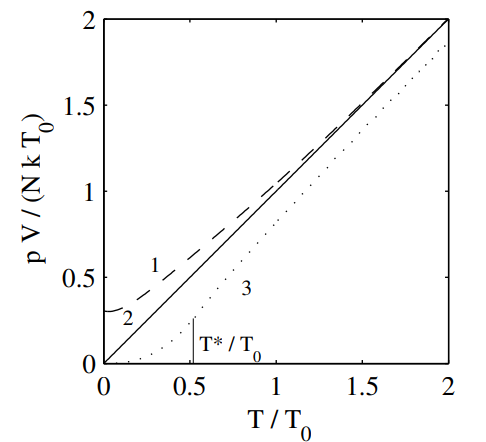
\includegraphics[scale=0.4]{TroisStatistiques.png}
\end{center}

\section{\'Etude de la sublimation}
Un gaz monoatomique et un solide cristallin, constitués des mêmes atomes sans spin de masse $m$ coexistent à l'équilibre dans une enceinte de volume $V$  à la température $T$. On néglige le volume du cristal par rapport à celui du gaz. La vapeur est assimilée à un gaz parfait classique. Le nombre total d’atomes est $N$, dont $N_g$ sont dans la phase gazeuse et $N_s=N-N_g$ en phase solide.

\question Rappeler l'expression de la fonction de partition canonique du gaz $Z_g(T, V, N_g)$, puis en déduire son énergie libre et sa pression. 

\begin{center} \vspace{-0.5cm}\line(1,0){0.2\textwidth} \vspace{-0.5cm}\end{center}

Dans le solide, les atomes sont situés aux noeuds discernables d’un réseau cristallin. Ils sont supposés indépendants
les uns des autres, le mouvement de chacun d’eux étant celui d’un oscillateur harmonique à 3 dimensions
(modèle d’Einstein). L'état d’un atome est caractérisé par 3 entiers positifs ou nuls $n_x$, $n_y$,
$n_z$ et son énergie est :
\begin{center}
$\epsilon_{{n_x,n_y,n_z}}=-\epsilon_0+\hbar \omega ( n_x+n_y+n_z+\frac{3}{2})$
\end{center}
où $\epsilon_0$ et $\omega$ sont des constantes caractéristiques du cristal.

\question Que représentent $\epsilon_0$ et $\omega$ ?

\question Exprimer la fonction de partition canonique du solide $Z_s(T, N_s)$. En déduire son énergie libre.

\begin{center} \vspace{-0.5cm}\line(1,0){0.2\textwidth} \vspace{-0.5cm}\end{center}

A priori, le nombre d’atomes sublimés $N_g$ peut prendre toutes les valeurs entre 0 et $N$. On se propose
de déterminer sa valeur à une température donnée.

\medskip

\question Comment s'écrit, en fonction de $Z_g$ et $Z_s$, la fonction de partition canonique de l'ensemble solide-gaz
en tenant compte de toutes les valeurs que $N_g$ peut prendre ?

\question Quelle est la probabilité pour que $N_g$ prenne une valeur particulière $N_g^0$ ?

\question En déduire la valeur la plus probable $N_g^E$ du nombre d'atomes dans la vapeur. Montrer qu'elle
correspond au cas où les potentiels chimiques des atomes dans le solide et dans le gaz sont égaux.

\question \`A température $T$ donnée, on s'intéresse aux variations de $N_g^E$ avec $V$. Montrer que pour $T$ et $N$ fixés, l'équilibre solide-vapeur n'est possible que si le volume $V$ de l’enceinte est inférieur à une certaine
valeur $V_M$ que l'on déterminera. Que se passe-t-il si on impose au système un volume $V$ supérieur à $V_M$ ?


\section{Gaz ultra-relativiste de bosons à 2D}

On considère un gaz parfait constitué de $N (\sim {\cal N}_A)$ bosons sans spin ultra-relativistes, {\bf indiscernables}, confinées sur une surface $A$ de dimension 2 à la température $T$ et au potentiel chimique $\mu$: l'énergie cinétique $\epsilon_i$ d'une particule $i$ est donnée par $\epsilon_i= p_ic$ où $c$ est la vitesse de la lumière et $p_i=|\Vec{p_i}|=\hbar |\Vec{k_i}|$ la norme de sa quantité de mouvement $\Vec{p_i}$ associée au vecteur d'onde $\Vec{k_i}$. On admet que la densité d'état dans l'espace réciproque (des vecteurs d'onde) est $\hat{\rho}(\Vec{k})d^2 \Vec{k}= \frac{A}{(2 \pi)^2} d^2 \Vec{k}$.

\question Montrer que la densité d'état en énergie $\rho_E(\epsilon)$ est de la forme $K \epsilon$ où $K$ s'exprime en fonction de $A, h$ et $c$. 

\question Rappeler l'expression du nombre moyen de particules $n_i^B(\epsilon)$ dans un état quantique $i$ d'énergie $\epsilon$ en fonction de $\beta, \epsilon$ et $\mu$.

\question \'Ecrire les expressions formelles dans l'approximation continue (sous forme d'intégrales sur l'énergie)  du nombre moyen de particules $N$ et de l'énergie moyenne $U$. On introduira $\alpha=N\frac{\Lambda^2}{A}$ où $\Lambda=\frac{h}{\sqrt{2\pi m k_B T}}$.

\question
Conclure quant à l'existence, ou l'absence d'un phénomène de condensation de Bose-Einstein pour des bosons ultrarelativistes en deux dimensions. On rappelle que
\begin{equation}
g_n(f)=\frac{1}{\Gamma (n)} \int_0^{+\infty} \frac{x^{n-1}\ dx}{\frac{\exp x}{f}-1}=\sum\limits_{p=1}^{+\infty} \frac{f^p}{p^n}.
\end{equation}

\end{document}
\section{\'Equation d'état d'un gaz parfait selon la statistique}

La figure ci-dessous présente les équations d'état de trois gaz parfaits non relativistes à trois
dimensions (numérotées de haut en bas). Les $N$ particules de masse $m$, confinées dans un volume $V$ sont supposées sans
structure interne. Le produit $pV$ et la température $T$ sont adimensionnés grâce à la température
caractéristique : $T_0=\frac{h^2}{2\pi m k_B} \left( \frac{N}{V} \right)^{\frac{2}{3}}.$



\question
Rappeler la définition de la longueur d'onde de De Broglie $\Lambda$ à la température $T$.
Quel est son sens physique ? En déduire une interprétation de la température caractéristique $T_0$.

\question \`A quelle statistique étudiée en cours chacune de ces trois courbes correspond-elle ?

\question Expliquer l'existence d’une ordonnée à l’origine non nulle pour la courbe 1. Donner un exemple de système physique qui vérifie cette équation d'état.

\question
Concernant la courbe 3, à quel phénomène physique
la température $T^*=\frac{T_0}{\zeta(\frac{3}{2})^{\frac{2}{3}}} \approx  0,52 \ T_0$ (indiquée par un trait vertical sur la figure) correspond-elle ? $\zeta(s)=\sum_{k=1}^{+\infty} \frac{1}{k^s}$ est la fonction zêta de Riemann. 

\question Pour $T \gg T_0$, les trois courbes se rejoignent. En pratique, la courbe 2 est-elle réaliste à basse température ? Pourquoi ?

\begin{center}
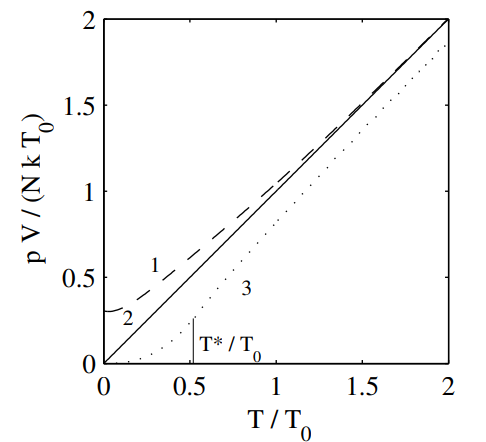
\includegraphics[scale=0.4]{TroisStatistiques.png}
\end{center}